%%%%%%%%%%%%%%%%%%%%%%%%%%%%%%%%%%%%%%%%%
\documentclass{article} % 'openany' here removes the gap page between days, erase it to restore this gap; 'oneside' can also be added to remove the shift that odd pages have to the right for easier reading

\usepackage[margin=1.00in]{geometry}

\usepackage[
  backref=page,
  pdfpagelabels=true,
  plainpages=false,
  colorlinks=true,
  bookmarks=true,
  pdfview=FitB]{hyperref} % Required for the hyperlinks within the PDF

\usepackage{booktabs} % Required for the top and bottom rules in the table
\usepackage{float} % Required for specifying the exact location of a figure or table
\usepackage{graphicx} % Required for including images2
\usepackage{lipsum} % Used for inserting dummy 'Lorem ipsum' text into the template
\usepackage{subfigure}
\newcommand{\HRule}{\rule{\linewidth}{0.5mm}} % Command to make the lines in the title page
\setlength\parindent{0pt} % Removes all indentation from paragraphs



%---------------------------------------------------------------------------------------
%%% TO ADD MATLAB FILES %%%%%
\usepackage{listings}
\lstset{basicstyle=\ttfamily\footnotesize,breaklines=true}
\usepackage{color} %red, green, blue, yellow, cyan, magenta, black, white
\definecolor{mygreen}{RGB}{28,172,0} % color values Red, Green, Blue
\definecolor{mylilas}{RGB}{170,55,241}
%%%%%%%%%%%%%%%%%%%%%%%%%%%%%
\usepackage{wrapfig}
\begin{document}

% ---------------- TO ADD MATLAB FILES --------
\lstset{language=Matlab,%
    %basicstyle=\color{red},
    breaklines=true,%
    morekeywords={matlab2tikz},
    keywordstyle=\color{blue},%
    morekeywords=[2]{1}, keywordstyle=[2]{\color{black}},
    identifierstyle=\color{black},%
    stringstyle=\color{mylilas},
    commentstyle=\color{mygreen},%
    showstringspaces=false,%without this there will be a symbol in the places where there is a space
    numbers=left,%
    numberstyle={\tiny \color{black}},% size of the numbers
    numbersep=9pt, % this defines how far the numbers are from the text
    emph=[1]{for,end,break},emphstyle=[1]\color{red}, %some words to emphasise
    %emph=[2]{word1,word2}, emphstyle=[2]{style},
}
%%%%%%%%%%%%%%%%%%%%%%%%%%%%%%%%%%%%%%%%%%%%%%%

%----------------------------------------------------------------------------------------
%	TITLE PAGE
%----------------------------------------------------------------------------------------

%\frontmatter % Use Roman numerals for page numbers
\title{
\begin{center}
\HRule \\[0.4cm]
{\Huge \bfseries Experiment 5:  Custom Orifice Plate Flow Sensor \\[0.5cm] \Large ME-330}\\[0.4cm] % Degree
\HRule \\[1.5cm]
\end{center}
}
\author{\Huge Dr. Vibahv Durgesh \\ \\ \LARGE vdurgesh@uidaho.edu \\[2cm]} % Your name and email address
\date{Week-04} % Beginning date
\maketitle

\tableofcontents

\clearpage



\section{Learning objective}
The objectives of this experiment are to provide the student with an opportunity to:

\begin{itemize}
\item	Calibrate a custom orifice plate using a rotameter as a reference standard.
\item	Observe the dynamic response of piezoelectric pressure sensors during flow rate changes.
\item	Gain experience with nonlinear regression (curve fitting).
\item	Use regressed calibration curve to create a flow measurement system.
\end{itemize}

\section{Equipment checklist}
\begin{wrapfigure}{r}{0.2\textwidth}
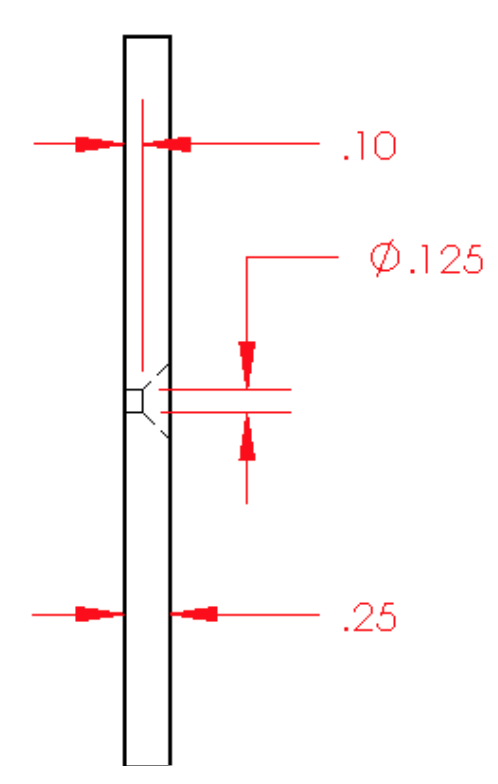
\includegraphics[width=1.25in]{Lab05Fig01.png}
\caption{Orifice plate internal geometry. Flow is from left to right.}
\label{fig:orficePlate}
\end{wrapfigure}
\begin{itemize}
\item	Air flow apparatus with Kings Rotameter and custom orifice plate with up- and down-stream pressure taps.
\item	One Honeywell differential pressure sensors with $\pm$30 psi range (P/N SSCDRRN030PDAA5) and two air hoses.
\item	Benchtop power supply.
\item	Wire Kit, Wire Strippers, Pliers, Screwdriver.
\item	Digital Multi-Meter (DMM).
\item	Data acquisition device NI-USB6008
\end{itemize}

\section{Introduction}

Orifice plates and rotameters are two common types of flow sensors. Rotameters are displacement volume flow sensors; they measure flow by observing the displacement of a float in an upwards flow stream. For this experiment, a purchased rotameter is provided as the flow measurement standard. More details are given in the References.\\
Orifice plates are obstruction flow sensors; they measure the difference between upstream and downstream pressure caused by an obstruction in the flow stream. For orifice plates, the obstruction is a plate with a hole that is smaller than the existing flow pipe. The obstruction causes a pressure drop. For this experiment, a custom orifice plate with pressure taps has been provided.  The orifice plate internal geometry is shown in figure \ref{fig:orficePlate}. \\
To create a custom orifice plate flowmeter, downstream and upstream pressure will be measured separately with two Honeywell pressure sensors. Then, differential pressure (the pressure drop across the flowmeter) can be correlated to the flow measured by the rotameter to create a calibrated flow measurement system.
Flow through an obstruction meter, such as an orifice plate, can be calculated according to:
\begin{equation}
Q= \left( Y K_{o}A_{o}\sqrt{\frac{2}{\rho}} \right) \sqrt{\Delta P},
\label{eq:calA}
\end{equation}
where $\Delta P$ is the pressure drop, $\rho$ is the density, $A_o$ is the throat area, $K_o$ is the flow coefficient, and $Y$ is the adiabatic expansion factor (compressible fluids only).  In this experiment the calibration equation will have the form:
\begin{equation}
Q = a_1 \sqrt{\Delta P} + a_o
\label{eq:calB}
\end{equation}
where $a_1$ will be the best estimate of the combined factor $Y K_{o}A_{o}\sqrt{\Delta P}$ and   should be close to zero.  This regression can be performed by plotting the measured flowrate vs the square root of the measured pressure drop and then using Matlab’s fitting function (polyfit).
\section{Laboratory instruction}
The goal of this experiment is to create a custom measurement system that indicates air flow based on pressure drop measurement across a custom orifice plate apparatus.
%\section{Part-A}
%\emph{Create a Matlab program to measure voltage output from pressure.}
%\begin{itemize}
%\item Create a Matlab program to acquire data from pressure sensor.
%\item Use a sampling rate of 200 Hz (change if mentioned otherwise)
%\item The output voltage from sensor is proportional to the pressure drop voltage across the orifice plate.
%\item Make sure to {\bf subtract the pressure voltage at zero flow rate condition} to all the measured differential pressure voltage.
%\end{itemize}


\section{Part-A}
\emph{Connecting the sensor and hardware}
In this lab you will be using two Honeywell SSCDRRN030PDAA5 pressure sensors (see Figure 2) with analog output. These differential pressure sensors have a $\pm$30 psi range, require a 5V supply and are amplified and temperature compensated. For more information, see \href{https://sensing.honeywell.com/SSCDRRN030PDAA5-amplified-board-mount-pressure-sensors}{Honeywell pressure transducer SSCDRRN030PDAA5 webpage}.
A single apparatus will serve two stations; you will work with a group directly across from your station. Each station will have its own data acquisition but the flow apparatus, pressure sensors, and breadboard circuit will be  shared and common. Please make sure to plan accordingly.

\begin{itemize}
\item Place pressure sensors on the breadboard. A sample connect for the components on a breadboard is shown in Figure \ref{fig:sampleCon}.
\item Supply each pressure sensor with a 5V supply and ground wire. Reference the Figure \ref{fig:sampleCon} for the proper pinouts. {\bf Do not turn on the power supply until confirming your circuit with the TAs.}
\item Using the supplied air hose, connect each pressure tap on the experimental apparatus to Port 1 on each pressure sensor. Port 1 is the ``Pressure Port'' and Port 2 is the ``Reference Port''. Thus each pressure sensor will measure differential pressure between the ports.  What is this pressure called? See Figure \ref{fig:sampleCon2} for proper experimental setup.
\item Connect the output voltage from the sensor to differential inputs on the NI-USB6008. Connect both Vout and GND.
\item Show the connections to the TAs prior to switching on the power supply.
\item Use the Matlab acquisition program to check the output (see the code in the appendix \ref{app:mainDAQProgram}. TAs should be able to verify the output values are correct or not. Before running the code make the following changes
    \begin{itemize}
      \item Make sure to set the sampling time for 10 seconds
      \item Set the sampling rate of 100 Hz
      \item Make sure the name the file ``trial.dat''
      \item For this part of the experiment you should keep the slope = 1, intercept =0, and $V_0=0.00$; in the Matlab program.
    \end{itemize}
\end{itemize}

\begin{figure}
\centering

\includegraphics[width=6.00in]{Lab05Circuit03.png}
\caption{Sample connection for experiment 4.}
\label{fig:sampleCon}
\end{figure}

\begin{figure}
\centering
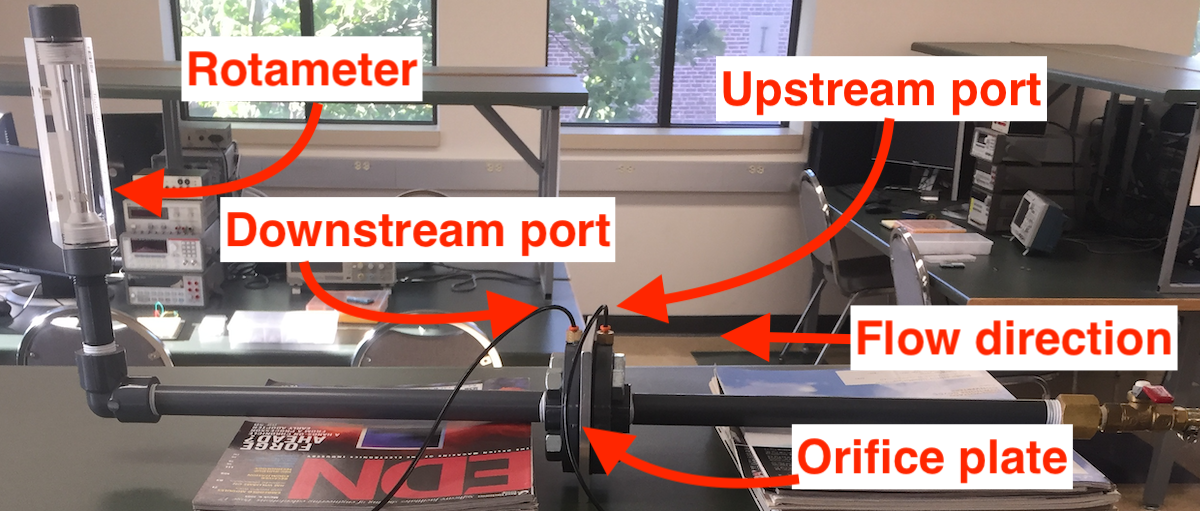
\includegraphics[width=5.00in]{Lab05OrificePlate.png}
\caption{Experimental setup for orifice plate.}
\label{fig:sampleCon2}
\end{figure}



\section{Part-B: Record calibration data}
In this lab we will be using a Kings’ Rotameter as a reference for flow rate. These rotameters measure air flow by correlation to vertical displacement of a float in the flow field (the rotameter must be vertical during measurements). Inspect the rotameter for flow units and proper reading technique. Additional information for the King's rotameter see website \href{https://kinginstrumentco.com/glass-flowmeters/}{Rotameter}.
During this part, you will work together with the station directly across from your station. Identify one person to vary the flow, one to read the rotameter, and one from each station to record the pressure sensor voltages from Matlab and the flow data from the rotameter


\begin{itemize}
\item Flow rate is controlled through a ball valve located between the air supply hose and the apparatus. Open the valve slightly to test your circuit and calibration Matlab program. See the Matlab calibration program \ref{app:calCode}.
\item Verify your circuit and setup with the TAs.
\item Procedure for calibration. (Make sure you have atleast ten points for calibration.)
\begin{itemize}
\item Open the valve - to obtain a desired flow rate. Make sure to take care of parallax error and use the right readout location for float.
\item Wait for atleast 10 seconds. The will allow time for the flow and pressures to settle to their nominal value.
\item Start you Matlab calibration program. Acquire data for 20 seconds and sampling rate of 30 data per second
\item Record the flow rate from Rotameter and corresponding average output voltage (shown on top the figure file of your calibration plot) in your log book.
\item First data point in your calibration will should be for zero flow rate condition (i.e., valve fully closed).
\item Take at least ten points evenly distributed across the flow range of the apparatus.
\item You will use the recorded  data from your log book to the matlab program to generate your calibration curve.
\end{itemize}
\item Note: {\bf subtract the voltage for zero flow rate case for all the other calibration data, while performing calibration}.
\item For the calibration you will values from first and third column of data, as shown in table \ref{tab:calData}.
\item A sample data used for calibration is shown in table \ref{tab:calData}. Make sure to have a similar table in your log book.
\item Plot your calibration data (i.e, calibration data recorded in your log book).  Is it linear or nonlinear?  Inspect your plot to identify if additional measurements are needed to provide a good calibration. A sample calibration plot is shown in Figure \ref{fig:sampCalPlot}.
\item Write down your calibration slope value and intercept value in the log book. These values will be used for other parts of your experiment.
\end{itemize}
\begin{table}
\centering
\caption{Sample calibration data.}
\begin{tabular}{c|cc}
Flow rate (scfm) & Voltage (v) & Voltage - $V_{zero, flowrate}$ (v)\\\toprule
0 & 2.5534 & 0 \\
1.0 & 2.5806 & 0.0272\\
1.6 & 2.6379 & 0.0845\\
2.0 & 2.6783 & 0.1249 \\
2.6 & 2.7503 & 0.1969 \\
3.0 & 2.8058 & 0.2524\\
3.6 & 2.9352 & 0.3818\\
4.0 & 3.0423 & 0.4889\\
4.6 & 3.2088 & 0.6554\\
5.0 & 3.3549 & 0.8015\\
5.6 & 3.5643 & 1.0109\\
6.0 & 3.6940 & 1.1408\\
\end{tabular}
\label{tab:calData}
\end{table}

\section{Part-C: Custom Orifice plate flowmeter calibration}
\begin{itemize}
\item Once calibration data collection is complete, plot the data in Matlab.  Make sure to plot the measured flowrate vs the square root of the measured pressure drop. See sample program to plot the calibration data is provided in appendix \ref{app:pltCalibration}.
\item Using the polyfit function in Matlab, perform a linear calibration. The determined slope and bias will correspond to   and  defined in equation \ref{eq:calB}.
\item For your post lab report, create side-by side plots using Matlab’s subplot command. Each subplot should have a series of data points plotted as markers and a calibration line/curve as a line.  See sample calibration plot in Figure \ref{fig:sampCalPlot}. Make sure to have a similar plot for your calibration.
\item {\bf LEFT PLOT:}  Use markers to plot your measured flow rate vs. the square root of the pressure drop.  Also include your linear fit line from the regression. The plot should include axis labels (with units), a legend, etc. Also show the 95\% confidence level for the curve fit.
\item {\bf RIGHT PLOT:} Use markers to plot your measured flow rate vs. the pressure drop (NOT THE SQUARE ROOT OF PRESSURE DROP). Then, generate your calibration curve by creating a list of pressure drops over the calibration range and calculating the calibrated flow using your calibration equation \ref{eq:calB}.
\end{itemize}
\begin{figure}
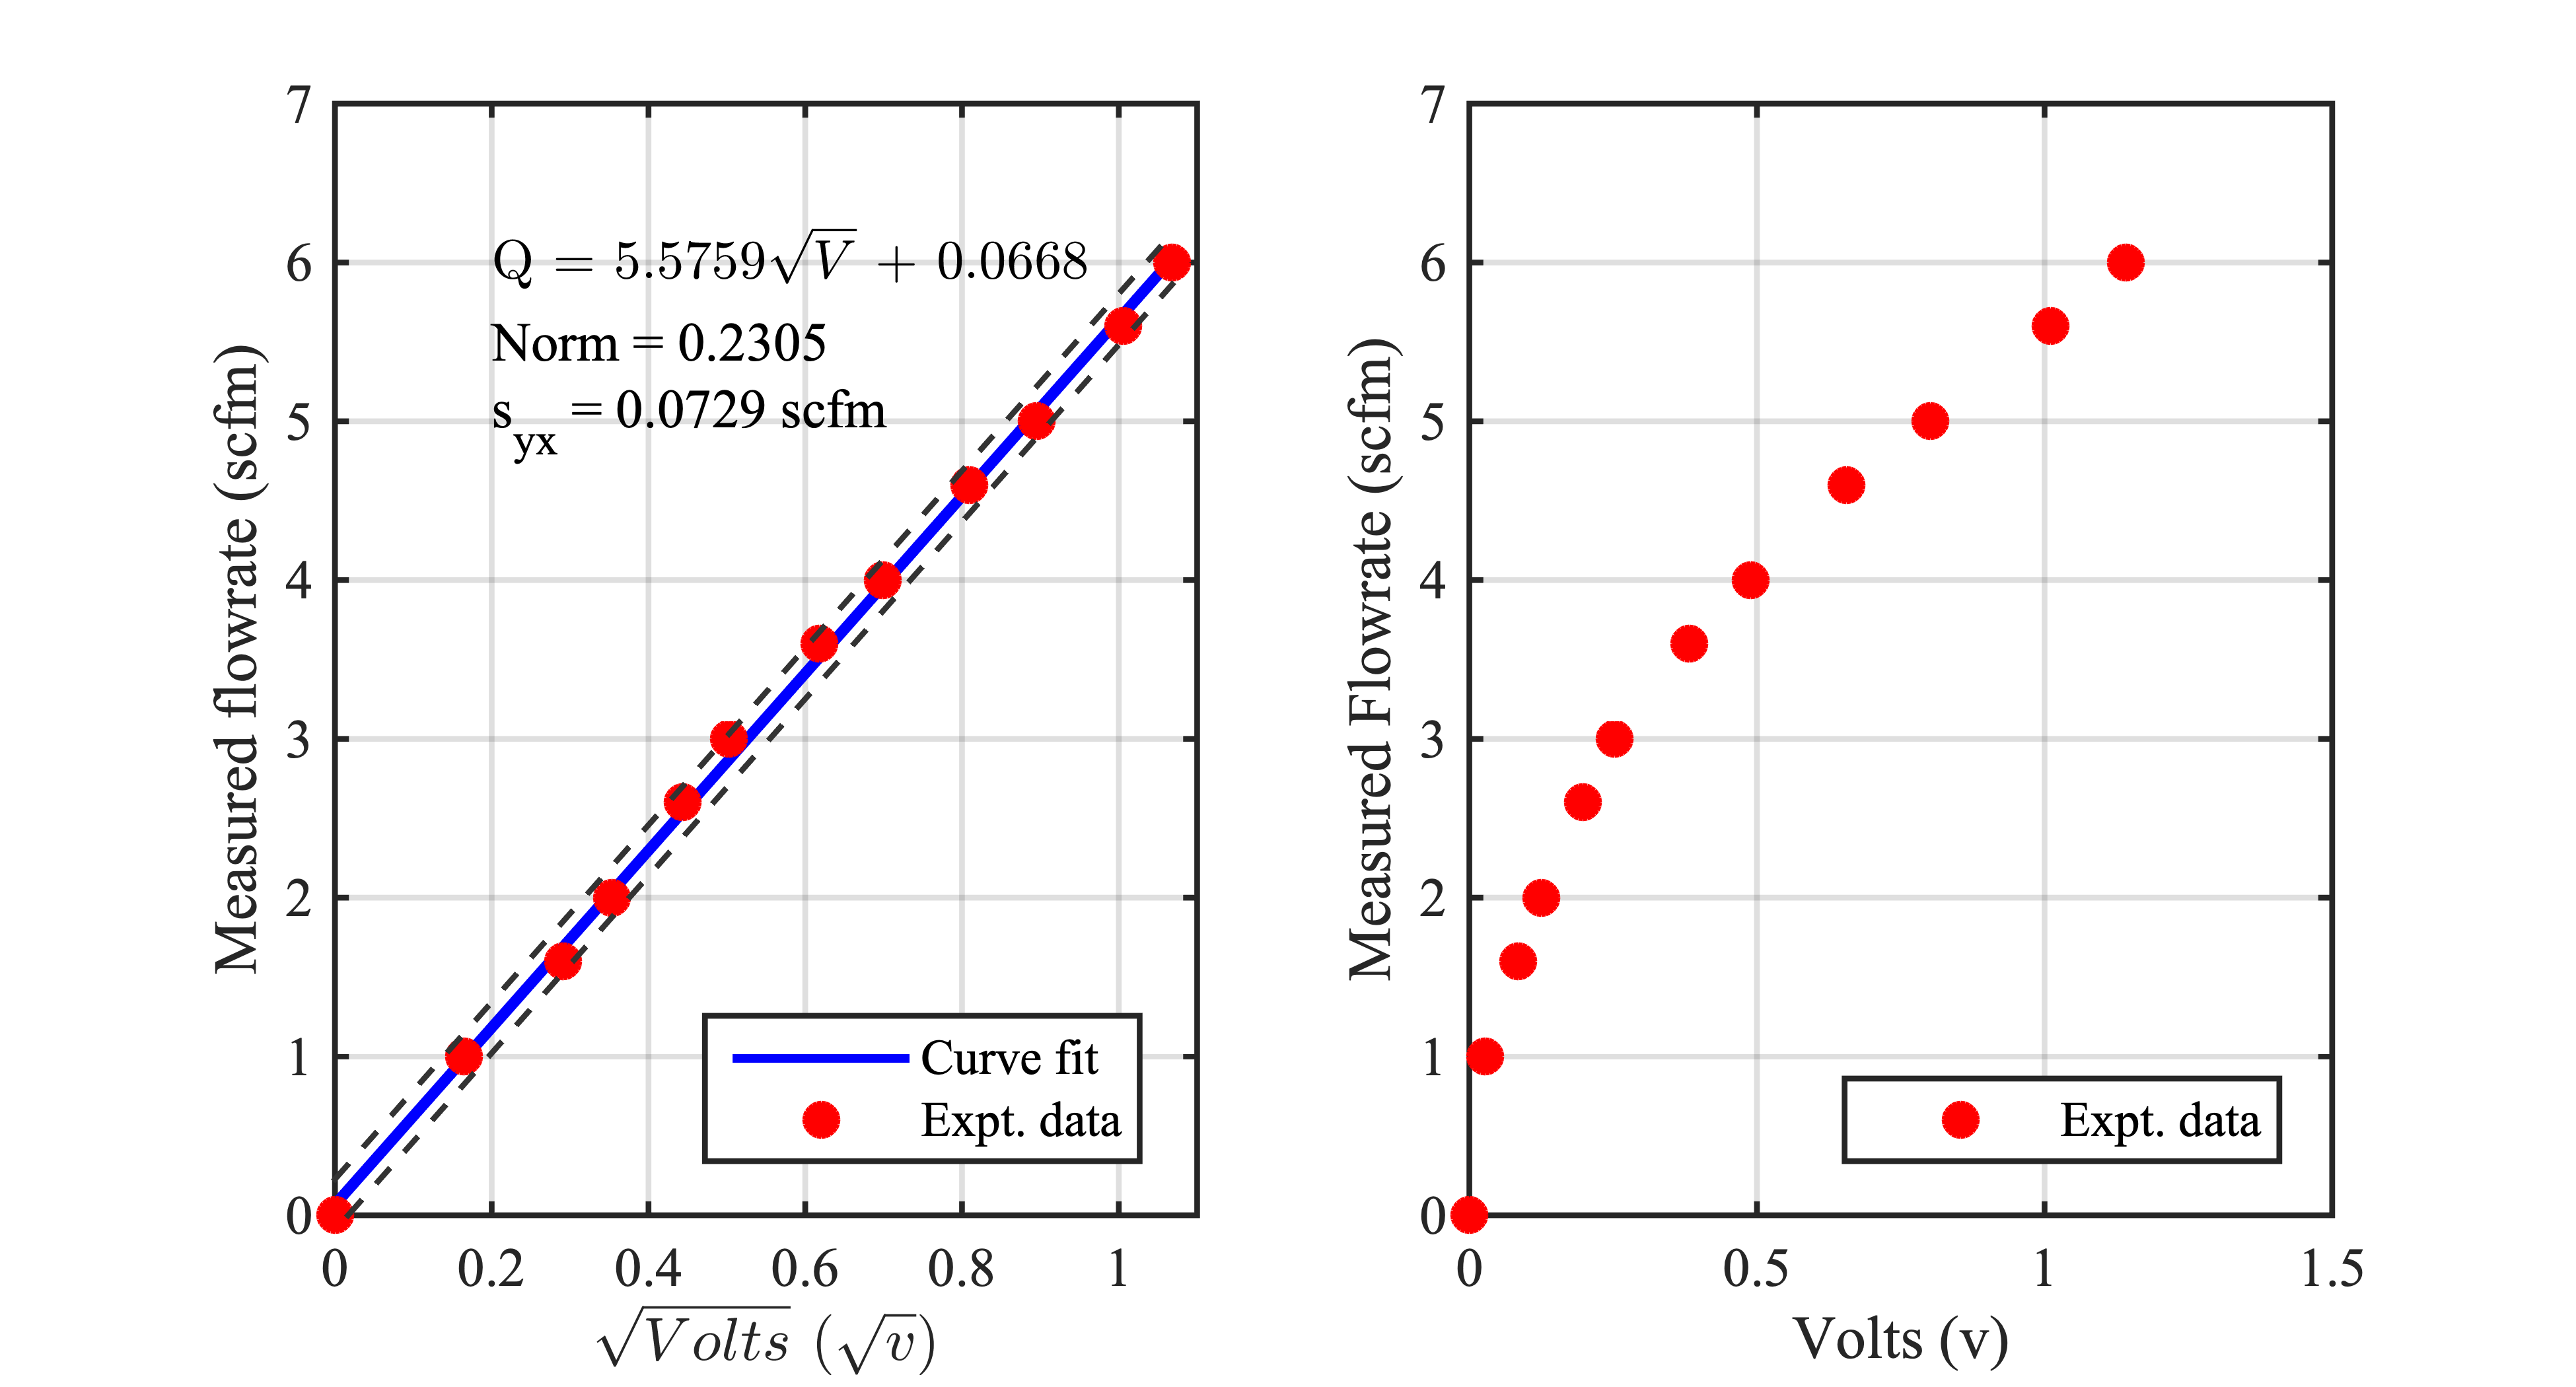
\includegraphics[width=6.0in]{Firstname_Lastname_Exp05_CalPlot.png}
\caption{Sample calibration plot with all the relevant details.}
\label{fig:sampCalPlot}
\end{figure}

\section{Part-D: Custom Orifice plate flowmeter verification.}
\emph{ Verification should be performed five distinct flow rates.}
\begin{itemize}
\item Program your calibration equation into main acquisition program (see code in appendix \ref{app:mainDAQProgram}). Make sure to input correct slope and intercept values in the program (use the value written in your log book). {\bf Also set $V_0$ in your Matlab program to the voltage value obtained for zero flow rate condition (see the table in your log book)}.
\item Open the values to get a desired flow rate and wait for 10 seconds for the rotameter reading to stablize.
\item Start your DAQ program. Collect data for 20 seconds at sampling rate of 200 Hz.
\item Compare your average calibrated flowrate indicated in from DAQ system to flowrate indicated by the Rotameter.
\item Make sure to check your recorded data file. It should store file in three columns: first column is time data, second column is voltage data and the third column is flow rate data.
\item Record the rotameter reading and average flow rate reading from DAQ system in your logbook.
\item Repeat this at five distinct flow rates, recording both flowrates (from the DAQ and from the Rotameter).
\item How accurate is your calibration?
\item Is it an accurate flow measurement?
\item Is it repeatable?
\end{itemize}


\section{Part-E: Record flowrate vs time for a step input of the ball valve}
\begin{itemize}
\item Set your Matlab program to acquire data for 7 seconds. With a sampling rate of 1000Hz. Here you can use the same Matlab program used in the previous part. You may have to modify the acquistion time and sampling rate. The calibration values, and $V_0$ values should remain same.
\item Close the inlet valve. Start recording in Matlab DAQ program.
\item Open the valve all the way at approximately at 2 second. Repeat as needed for timing.
\item Make sure to save this time series data for plotting.
\item Save both raw voltage data and the flow rate after (i.e., using the calibration values).
\item Is there a significant transient response?
\item Is there overshoot? Do you think the flowrate calibration is valid during the transient response?  Is the pressure drop during the transient response within the calibration range?
\item Create a plot with two y-axis scales using plotyy: the left y-axis should be in volts for the pressure drop voltage and the right y-axis should be in the calibrated flow units (SCFM).  Plot both pressure drop and calibrated flow rate vs time for the 5 second step response. See the program in appendix \ref{app:postLabTrans}.
\end{itemize}
A sample plot for the transient response is show in figure \ref{fig:trRes}. Make sure to have similar plot for your report.
\begin{figure}[!ht]
  \centering
  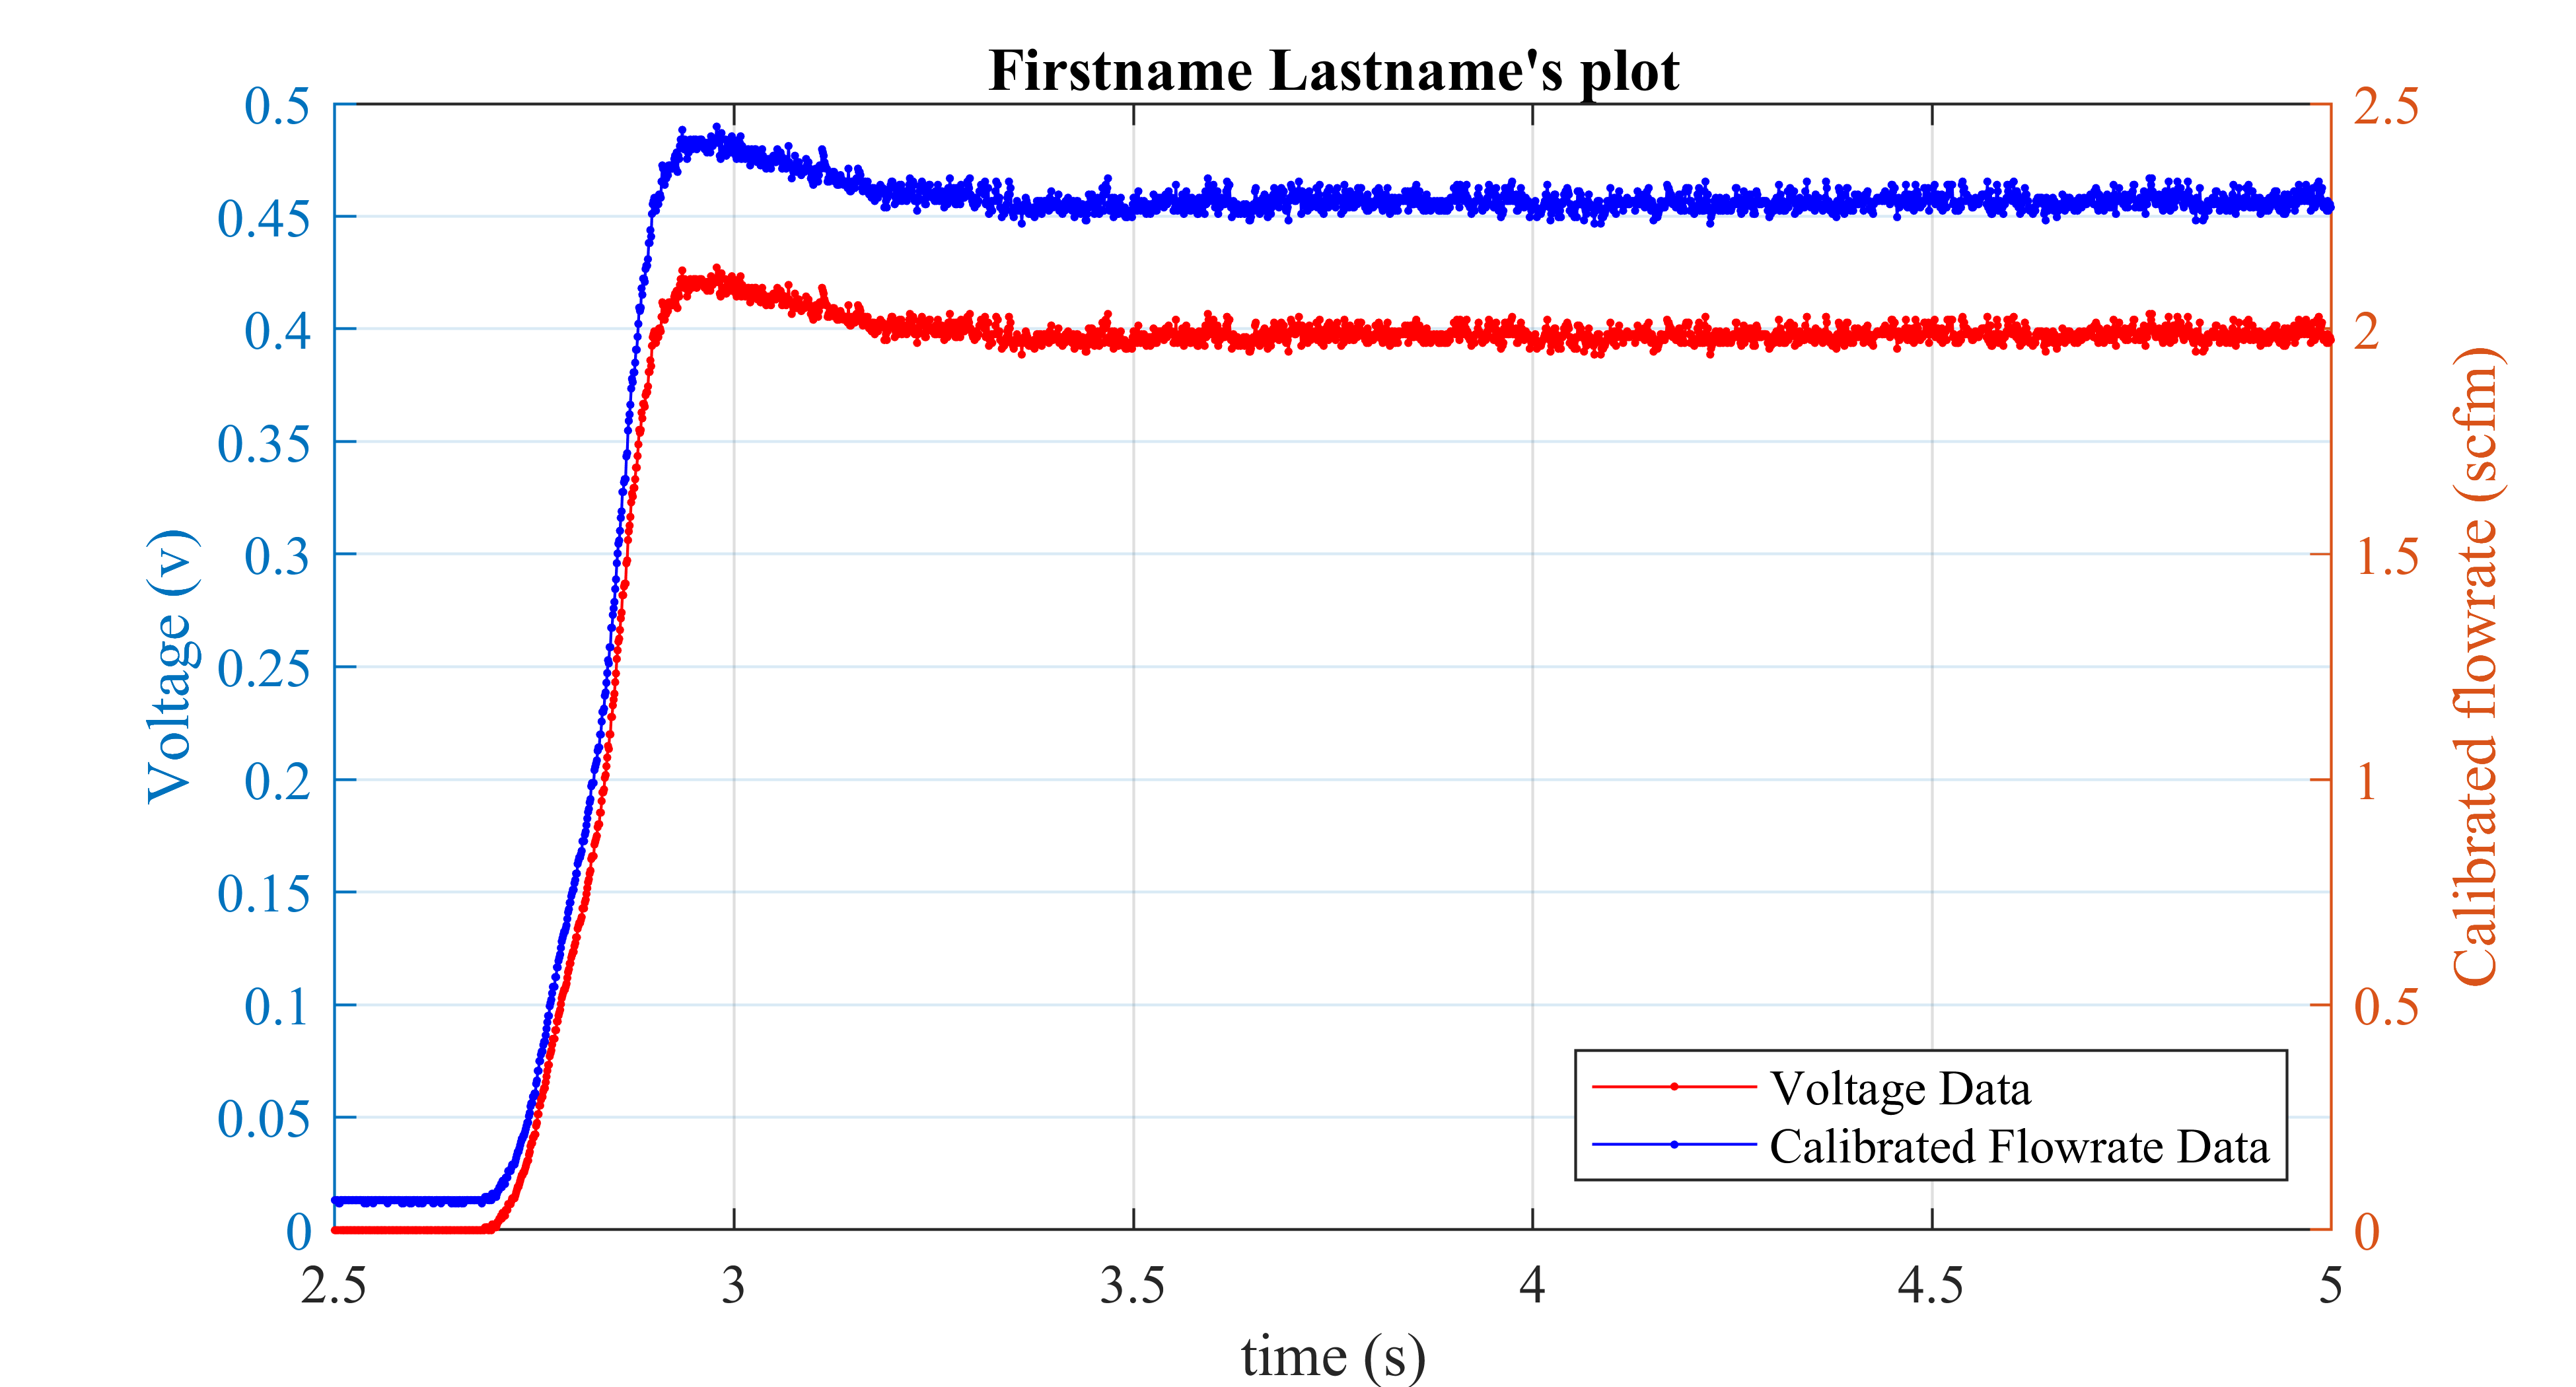
\includegraphics[width=6.00in]{Firstname_Lastname_Exp05_Part2.png}
  \caption{Sample transient response plot}
  \label{fig:trRes}
\end{figure}


\section{Part-F}
Return lab space to prior condition
\begin{itemize}
\item Turn off the power supply.
\item Remove wires connecting the power supply to the breadboard and return to the wall
\item Remove all breadboard wires and place them back in the wire kit in an organized fashion.
\item Remove the pendulum wires from the breadboard and set aside.
\item Log off the computer.
\item Make sure to copy the data to your harddrive.
\item {\bf Do this for every lab!}
\end{itemize}

\section{Part-G}
\emph{For this experiment submit the following items on BbLearn for your post-laboratory assessment.}
\begin{itemize}
\item Custom orifice plate calibration plots. Submit a single figure with side-by-side calibration plots .
\item Step input response plot. Submit the time series plot.
\end{itemize}

\section{Post-Laboratory Report}
This experiment will be the subject of the 1st of 3 Formal Reports.  For this first report, start with the report draft posted on BbLearn.


\section{Appendix}
%
%
\subsection{Matlab program to calibrate pressure sensors}
\label{app:calCode}
\lstinputlisting{../MatlabProgram/mainAcqProgram_ForCalibration.m}
%%
\clearpage
\subsection{Matlab program to plot calibration data}
\label{app:pltCalibration}
\lstinputlisting{../MatlabProgram/generate_CalibrationPlot.m}
%%
\clearpage
\subsection{Matlab program to acquire data after your calibration}
\label{app:mainDAQProgram}
\lstinputlisting{../MatlabProgram/mainAcqProgram_ForCollectingData.m}
%
\clearpage
\subsection{Matlab program to plot transient response}
\label{app:postLabTrans}
\lstinputlisting{../MatlabProgram/Lab05_PostLab.m}
%\clearpage
%
%\subsection{Plot sample post lab}
%\label{app:postLabB}
%\begin{figure}[!ht]
%\centering
%
\includegraphics[width=5.0in]{Firstname_Lastname_Exp04_Part2.png}
%\caption{Sample plot dynamic signal post lab.}
%\label{fig:dynSignalPlot}
%\end{figure}
%\clearpage


\end{document} 